\chapter{Profilo dell'Agenzia}
\label{1.0}
\thispagestyle{fancy} 

ARPAV\ped{g} è l'agenzia regionale per la prevenzione e protezione ambientale del Veneto, operativa dal 3 Ottobre 1997 in seguito alla Legge Regionale n32° del 18 Ottobre 1996.

\begin{figure}[htbp]
	\centering
	
\includegraphics[scale=0.7]{./capitoli/capitolo1/img/logoARPAV.jpg}
	\caption{logo dell'agenzia}
\end{figure}

Le attività competenti riguardano la tutela, il controllo, il recupero dell'ambiente e per la prevenzione e promozione della salute collettiva al fine di conseguire la massima efficacia nell'individuazione e nella rimozione dei fattori di rischio per l'uomo e per l'ambiente. Le funzioni principale dell'agenzia riguardano attività tecnico-scientifiche per il monitoraggio, tutela e prevenzione di acqua, aria (inquinamento acustico ed elettromagnetico negli ambienti di vita), suolo, rifiuti solidi e liquidi, radioattività ambientale ed infine ai rischi di incidenti rilevanti attività industriali. L'esercizio delle attività di monitoraggio e prevenzione vengono effettuate in coordinazione con le unità locali socio sanitarie.\\
L'agenzia è suddivisa in vari organi operativi, i quali hanno funzionalità specifiche a seconda del ruolo che ricoprono. La suddivisione degli incarichi e delle competenze e la corretta comunicazione fra i vari dipartimenti, permette di gestire questo vasto ente in modo efficiente e sistematico.\\
Lo \textit{stage} in oggetto è stato svolto presso il servizio informatico e di reti. In questa sede vengono svolte le mansioni per la gestione dell'infrastruttura informatica e delle risorse strumentali hardware di tutta l'agenzia e attività di ricerca e sviluppo inerenti.

\begin{table}[htbp]
\centering
\begin{tabular}{|p{0.95\textwidth}|}
\hline

\begin{itemize}

    \item gestione e coordinamento delle banche dati dell'agenzia;
	
	\item assistenza sulle applicazioni informatiche dell'agenzia;
	
	\item definizione degli indicatori ambientali e dei rapporti;
	
	\item fornitura degli standard operativi, architetture delle realizzazioni, attivazione e gestione tecnica dei portali internet/intranet;
	
	\item gestione connettività aziendale, voce dati;
	
	\item gestione tecnico operativa per il funzionamento, la manutenzione e la connettività delle reti di monitoraggio dell'azienda.
\end{itemize}
	\\
	
\hline
\end{tabular}
\caption{mansioni dipartimento Servizio Informatico e Reti}
\end{table}

\section{Cosa offre: Prodotti e Servizi}

In questa sezione vengono elencati e descritti le tipologie di prodotti che ARPAV produce e i tipi diversi di servizi che offre, ponendo particolare attenzione a ciò che viene erogato dalla sede dello \textit{stage}.

\subsection{I Prodotti di ARPAV}

Non essendo un'azienda a scopo di lucro, ma un'agenzia regionale, ARPAV è tenuta alla parità di bilancio. L'orientamento generale non è propenso alla distribuzione e vendita di prodotti quindi, ARPAV, per lo più, collabora con altre aziende o enti per realizzare progetti in ambito ambientale come \textit{patner, subcontractor\ped{g}} o \textit{leader}.



\begin{longtable}{ p{0.2\textwidth} | p{0.3\textwidth} | p{0.5\textwidth}}

\textbf{Logo}& \textbf{Ruolo \& Nome}&  \textbf{Descrizione}\\

 \endhead
\midrule
\vfill 
\includegraphics[scale=0.8]{./capitoli/capitolo1/img/alpini} & \vfill \textbf{{\color{Plum}Ruolo}: \textit{Patner}} \newline \vfill \textbf{{\color{ForestGreen}SedAlp}: Programma Spazio Alpino}  &
 Sviluppo e \textit{testing} di politiche e strumenti utili alla gestione integrata del trasporto di sedimenti nei bacini alpini al fine di ridurre il rischio legato al trasporto solido e allo stesso tempo di migliorare la condizione ecologica degli ambienti acquatici e ripararli e ridurre l'impatto ambientale creato dalle centrali idroelettriche. \textit{\href{http://www.alpine-space.eu/}{website}}\\
\midrule
\vfill 
\includegraphics[scale=0.7]{./capitoli/capitolo1/img/med} & \vfill \textbf{{\color{Plum}Ruolo}: \textit{Leader}} \newline \vfill \textbf{{\color{ForestGreen}CAIMANs}: Programma Med}  & Valutando l'impatto sulla qualità dell'aria da parte delle navi crociera e in generale delle navi passeggeri, il progetto mira a porre le basi per l'identificazione dei punti critici e per proporre orientamenti per futuri progetti e politiche trasnazionali che affrontino la mitigazione dell'inquinamento atmosferico dovuto al traffico navale passeggeri. \textit{\href{http://www.medmaritimeprojects.eu/section/caimans}{website}} \\
\midrule
\vfill 
\includegraphics[scale=0.7]{./capitoli/capitolo1/img/park} & \vfill \textbf{{\color{Plum}Ruolo}: \textit{Patner}} \newline \vfill \textbf{ {\color{ForestGreen}GuardEn}: Programma South East Europe } & Sviluppo e \textit{testing} di un possibile quadro di riferimento finalizzato al supporto di un programma di implementazione di locali strategie per la gestione e prevenzione del rischio ambientale legato all'attività agricola e agroalimentare. In particolare per i territori interessati dall'inquinamento del suolo e dell'acqua, da proporre per l'applicazione alle aziende del settore. \textit{\href{http://www.southeast-europe.net/en/}{website}}\\
\midrule
\vfill 
\includegraphics[scale=0.7]{./capitoli/capitolo1/img/interr} & \vfill \textbf{{\color{Plum}Ruolo}: \textit{Patner}} \newline \vfill \textbf{{\color{ForestGreen}3PClim}: Programma Interreg IV Italia – Austria} &   Aggiornamento della climatologia delle Alpi orientali, con la produzioni di cartografie tematiche, elaborazioni e proiezioni climatiche. \textit{\href{http://www.interreg.net/it/programma/programma.asp}{website}}\\
\midrule
\vfill 
\includegraphics[scale=0.7]{./capitoli/capitolo1/img/resmia} & \vfill \textbf{{\color{Plum}Ruolo}: \textit{Patner}} \newline \vfill \textbf{{\color{ForestGreen}RE.S.M.I.A.}: Programma POR – FESR Veneto} & Progetto pilota di ricerca industriale con l’obiettivo di potenziare ed integrare la rete di monitoraggio ambientale a disposizione di ARPAV. \textit{\href{http://www.resmia.eu/}{website}} \\
\bottomrule
\caption{progetti ARPAV}
\end{longtable}

Il dipartimento di informatica e reti, in collaborazione con CIVEN\ped{g}, durante il periodo stagistico stava seguendo con particolare attenzione \textbf{RE.S.M.I.A.}\ped{g}. Il progetto consiste nel potenziamento dell'infrastruttura delle stazioni di monitoraggio ambientale attualmente a disposizione di ARPAV, con la progettazione ed installazione di sensori. Il nuovo concetto di stazione farà uso di tecnologia WSN\ped{g}, applicativi \textit{Web-Based}\ped{g} e sarà caratterizzato dall'ottimizzazione della efficienza energetica del sistema. \\


Le finalità principali del progetto sono:
\begin{itemize}

	\item \textbf{minimizzazione dell'impatto ambientale dall'installazione delle stazioni di monitoraggio:} utilizzo di tecnologie per l'auto-alimentazione dell'impianto e utilizzo di tecnologie \textit{wireless} per ridurre al minimo l'invasione ambientale e con sperimentazione di nuovi sensori elettrochimici nanostrutturati per il monitoraggio in sito di metalli pesanti;
	\item \textbf{riduzione dei costi di produzioni ed installazione:} utilizzo di nuovi \textit{hardware} a basso costo con ottime prestazioni, bassa necessità di manutenzione e semplice installazione, anche in presenza di condizioni morfologiche del territorio estremamente critiche. Realizzazione di prodotti in grado di essere installati da qualunque persona, in particolare volontari sprovvisti di preparazione;
	\item \textbf{tutela dell'ambiente:} monitoraggio delle matrici ambientali anticipando anche le disposizioni legislative e ponendo attenzione alle tematiche sentite dall'opinione pubblica in tema di salute, quale ad esempio il monitoraggio di nanoparticelle in aria;
	\item \textbf{prevenzione dei rischi:} determinazione delle soglie minime di allarme dei parametri ambientali reperibili in tempi brevi per l'intero territorio della Regione del Veneto;

\end{itemize}

\begin{figure}[htbp]
\centering
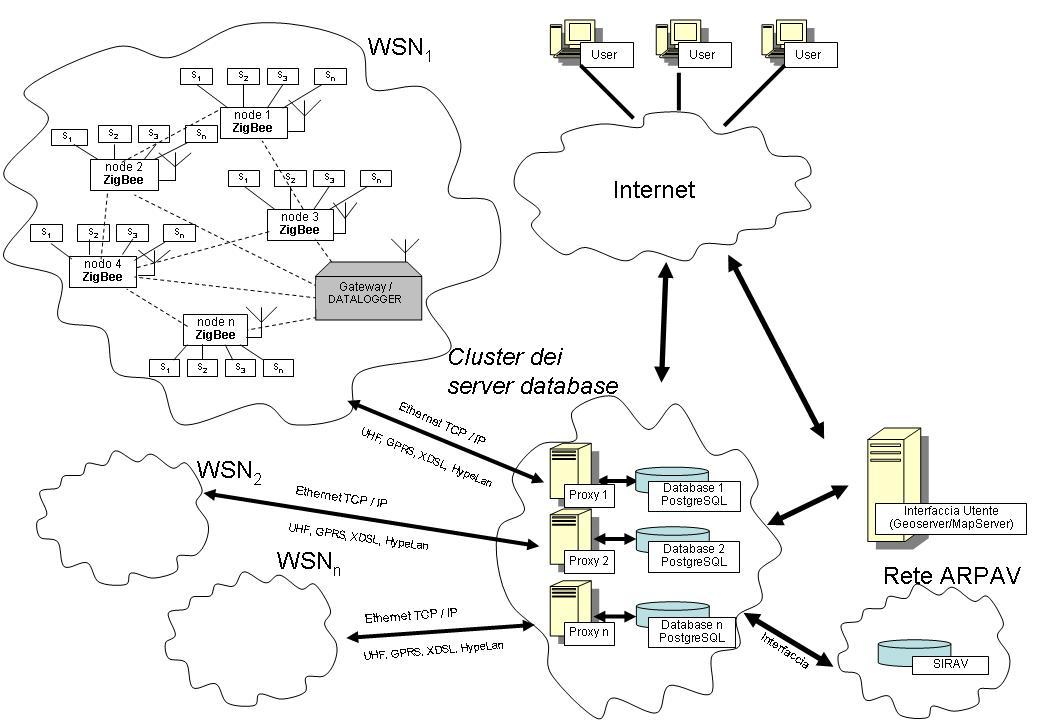
\includegraphics[scale=0.3]{./capitoli/capitolo1/img/retiresmia}
\caption{schema reti RESMIA}
\end{figure}

Il dipartimento di informatica e reti ha il compito di incrementare la struttura del sistema di salvataggio dei dati e di potenziare l'interfaccia \textit{web} che rappresenta graficamente su un'opportuna mappa la dislocazione dei sensori e ed effettuare opportune interrogazioni sui dati forniti tramite \textit{Map Server}\ped{g}.

\subsection{I Servizi di ARPAV}

L'agenzia regionale offre una vasta gamma di servizi, i quali possono essere suddivisi in due macro categorie: servizi ambientali e servizi online. I primi, offrono un servizio su richiesta o erogati da ARPAV, i secondi invece sono servizi passivi offerti dal portale \textit{internet}, i cui fruitori possono accedervi tramite \textit{network}.  \textit{\href{http://www.arpa.veneto.it/servizi-ambientali}{website}}

\subsubsection{Servizi Ambientali}

\begin{longtable}{ p{0.3\textwidth} | p{0.3\textwidth} | p{0.4\textwidth}}
\textbf{Nome}& \textbf{Possibili Fruitori}&  \textbf{Descrizione} \\
\endhead

	\midrule
	\textbf{{\color{OliveGreen}Acquisti pubblici verdi-GPP\ped{g}}} & Pubbliche amministrazioni locali o nazionali  & Informazione delle pubbliche amministrazioni circa l'adozione di pratiche d'acquisto verdi che riducono l'uso di risorse naturali, la produzione di rifiuti, i rischi ambientali \\
	\midrule
	\textbf{{\color{OliveGreen}Certificazioni ambientali}} & Imprese soprattutto piccole e medie &  Diffusione all'interno del mondo produttivo di una nuova cultura di sistema per la gestione consapevole ed ecocompatibile dell'ambiente attraverso lo sviluppo di progetti, strumenti, protocolli ad hoc\\
	\midrule
	\textbf{{\color{OliveGreen}Comunicazione}} & Cittadini & Promozione delle attività di educazione ed informazione ambientale dei cittadini \\
	\midrule
	\textbf{{\color{OliveGreen}Progetti \& Cooperazione}} & Aziende, imprese, enti pubblici o regioni & Avvio e realizzazione di progetti, avvio di relazioni internazionali generalmente finanziati da fondi dell'Unione Europea \\
	\midrule
	\textbf{{\color{OliveGreen} Grandi opere}} & Aziende coinvolte in appalti pubblici in Veneto & attività di audit preventivo e di monitoraggio ambientale per garantire la compatibilità ambientale, il corretto inserimento dal punto di vista urbanistico, ambientale, trasportistico e sociale delle Grandi Opere \\
	\midrule
	\textbf{{\color{OliveGreen} Educazione per la sostenibilità}} & Chiunque &  Attività di educazione, informazione e comunicazione ambientale, protezione della natura al fine di promuovere e sviluppare comportamenti sostenibili \\
	\midrule
	\textbf{{\color{OliveGreen} IPPC\ped{g} e  Servizi alle aziende}} & Aziende ed Imprese & Consulenze sul piano di monitoraggio e controllo in fase istruttoria per il rilascio dell'autorizzazione integrata ambientale, ispezioni integrate ambientali nelle aziende IPPC del Veneto\\
	\midrule
	\textbf{{\color{OliveGreen} Pronta disponibilità}} &  Dipartimenti di Prevenzione delle ULSS regionali Organi di polizia giudiziaria &  Attività di analisi immediata di aria, acqua e suolo secondo le modalità previste\\
	\midrule
	\textbf{{\color{OliveGreen} Rischio industriale}} & Industrie & Individuazione, classificazione e probabilità dei pericoli provenienti dalle industrie che utilizzano o detengono sostanze chimiche per le loro attività \\
	\midrule
	\textbf{{\color{OliveGreen} Sicurezza impiantistica}} & Comuni, ASL, Prefettura, Procura & Verifica della corretta funzionalità di impianti e macchinari installati in ambienti di lavoro o di vita e soggetti a controlli periodici \\
	\bottomrule
	

\caption{servizi ambientali ARPAV}
\end{longtable}

\subsubsection{Servizi Online}

\begin{longtable}{p{0.3\textwidth}|p{0.7\textwidth}}
\textbf{Nome} & \textbf{Descrizione} \\
\endhead

\midrule
\textbf{{\color{Plum} Accesso informazioni ambientali}} & Accesso del pubblico all'informazione ambientale detenuta o prodotta da soggetti pubblici avviene anche mediante l'utilizzo delle tecnologie informatiche e dei mezzi di telecomunicazione \\
\midrule
\textbf{{\color{Plum} Glossari Ambientali}} & Strumento di informazione aggiornata ed esaustiva che ARPAV mette a disposizione dei cittadini per favorire la comprensione di termini 'ambientali' maggiormente utilizzati \\
\midrule
\textbf{{\color{Plum} Iscrizione bollettini}} & Iscrizione alla mailing list consente di ricevere i bollettini Meteo direttamente nella propria casella di posta elettronica. Meteo Veneto, Dolomiti Meteo, Meteo Spiagge e Meteo Garda i bollettini per cui è disponibile il servizio \\
\midrule
\textbf{{\color{Plum} Iscrizione bollettini via sms}} & Sottoscrivendo un abbonamento è possibile ricevere via sms i contenuti di alcuni bollettini prodotti per l'area delle Dolomiti. Dolomiti meteo e Dolomiti Neve e Valanghe i bollettini per i quali è disponibile il servizio \\
\midrule
\textbf{{\color{Plum} Iscrizione \textit{newsletter}}} &  E' possibile ricevere periodicamente nella propria casella di posta le \textit{newsletter} con informazioni su eventi, contenuti e attività \\
\midrule
\textbf{{\color{Plum} Iscrizione applicativo web ORSO }} &  Programma per il monitoraggio del flusso dei rifiuti attraverso le Regioni d'Italia, con standard di riferimento comuni che garantiscano rappresentatività delle informazioni raccolte, oltre ad agevolare lo scambio di informazioni finalizzato alla corretta gestione dei rifiuti per i Comuni e gestori degli impianti \\
\midrule
\textbf{{\color{Plum} Iscrizione a IRRIFRAME}} & Servizio che permette alle aziende registrate di salvare il proprio profilo colturale e di personalizzare l'informazione irrigua fornita dal servizio comunicando in tempo reale dati locali \\
\midrule
\textbf{{\color{Plum} Link utili}} & Una rassegna di 'siti utili'; la suddivisione per argomenti e temi permette di individuare facilmente i riferimenti cercati \\
\midrule
\textbf{{\color{Plum} Richiesta pubblicazioni}} & Possibilità di richiedere una copia delle pubblicazioni edite da ARPAV attraverso posta elettronica e la compilazione di un modulo \\
\bottomrule

\caption{servizi online di ARPAV}
\end{longtable}

\newpage

\section{Organizzazione Interna}

ARPAV è un'agenzia regionale che lavora per il completamento di progetti a livello regionale, nazionale ed internazionale ed offre tutta una serie di servizi a livello regionale e non. Per fare ciò necessita di una  organizzazione interna ben strutturata, suddivisa in vari organi operativi, ognuno dei quali ricopre una funzionalità specifica e si interfaccia con un altra secondo protocolli prestabiliti. ARPAV è dotata di una autonomia interna negli ambiti amministrativi, organizzativi e tecnico contabile e di diverse figure professionali che garantiscono un approccio multidisciplinari.

\begin{figure}[htbp]
\centering
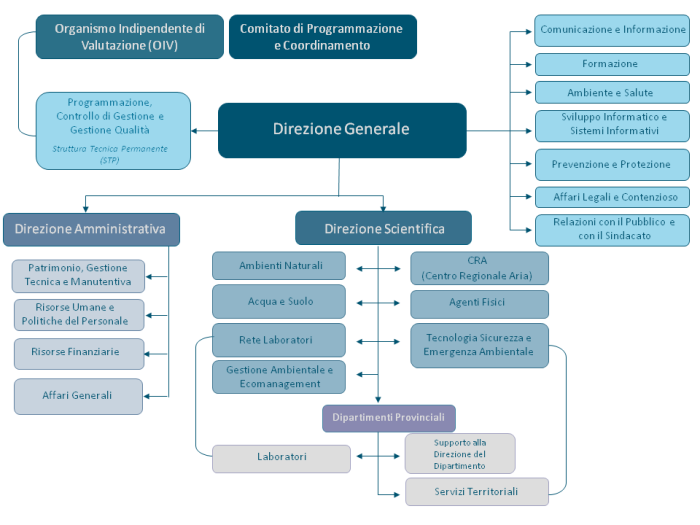
\includegraphics[scale=0.7]{./capitoli/capitolo1/img/organigramma}

\caption{organigramma struttura ARPAV}

\end{figure}

A livello macroscopico è composta da una \textbf{Direzione Generale}, che a sua volta si ramifica in più aree funzionali di natura amministrativa e tecnico-scientifica, due \textbf{Dipartimenti regionali} e sette \textbf{Dipartimenti provinciali}. I dipartimenti regionali e provinciali per la realizzazione dei programmi ed attività di competenza godono di una autonomia gestionale nei limiti delle risorse loro assegnate dalla direzione generale.\\
La sede dello stage si trova all'interno dell'area della \textbf{direzione amministrativa}, in particolare nel sottoinsieme della \textbf{gestione tecnica}.\\
L'organizzazione interna al dipartimento di informatica è riassumibile così:

\begin{figure}[htbp]
	\centering
	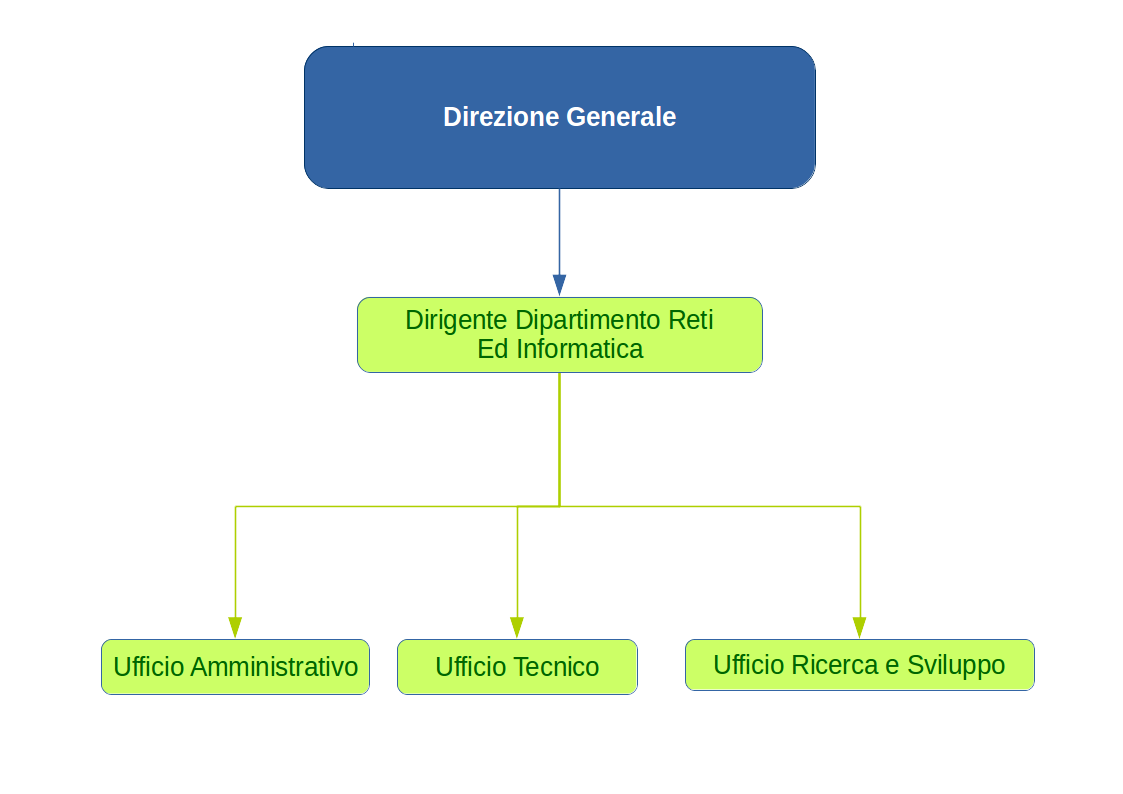
\includegraphics[scale=0.4]{./capitoli/capitolo1/img/organigrammaDip}
	\caption{organigramma Dipartimento Informatica e Reti}
\end{figure}

\begin{itemize}

	\item \textbf{Direttore:} figura a cui tutti fanno riferimento, ha il compito di relazionarsi con le aziende esterne per accordare collaborazioni nei progetti assegnati dalla \textbf{Direzione Generale}. Deve anche approvare i bilanci economici e gestire le risorse umane;
	\item \textbf{Ufficio Amministrativo:} ufficio con il compito di adempiere alle funzioni amministrative del dipartimento;
	\item \textbf{Ufficio di Ricerca e Sviluppo:} ufficio esecutivo in cui si sviluppano o si fa manutenzione sui progetti;
	\item \textbf{Ufficio Tecnico:} ufficio composto da tecnici addetti alla manutenzione del sistema di reti dell'intero ente.
	
\end{itemize}
\subsection{Processi di Sviluppo}

ARPAV svolge la propria attività sulla base un programma triennale. l responsabi
le della trasparenza predispone
il Programma triennale per la trasparenza e l’integrità per il
triennio 2012/2014
entro il 31/12/12
, e a tal fine
coordina il processo per la redazione del docume
nto
coinvolgendo le strutture responsabili della produzione dei dati oggetto di pubblicazione

 Il \textbf{Direttore Generale} predispone il piano di attività pluriennale di attività di ARPAV, sulla base degli obiettivi generali di monitoraggio e prevenzione ambientale. Il piano, acquisito il parere del comitato regionale di indirizzo e della competente commissione consiliare, viene approvato dalla Giunta regionale e ha di norma validità triennale. \\
Il Direttore Generale, inoltre, tenuto conto delle proposte dei \textit{comitati provinciali di coordinamento}\ped{g}, sulla base del del piano pluriennale approva il programma annuale di ARPAV, il quale deve contenere anche idonei interventi di educazione ed informazione volti alla tutela ambientale.

\begin{longtable}{p{0.2\textwidth}|p{0.3\textwidth}|p{0.5\textwidth}}
\textbf{Fase} & \textbf{Attività} & \textbf{Soggetti responsabili \& Compiti} \\
\midrule

\endhead



\multirow{3}{0.2\textwidth}{ \vfill Elaborazione / aggiornamento del
Programma triennale} 
	& Promozione e coordinamento del processo di formazione del Programma 
	& \textbf{{\color{Plum}Direttori della Direzione Centrale}:} (avvia il processo e fornisce gli indirizzi);
	\newline
	\textbf{{\color{Plum} Responsabile della trasparenza}:} (promuove e cura il coinvolgimento delle strutture interne);
	\newline
	\textbf{{\color{Plum}OIV\ped{g}}:}
 (prende consapevolezza dell'inizio delle attività) \\ \cline{2-3}
 & Individuazione dei contenuti del Programma 
 & \textbf{{\color{Plum}Direttori della Direzione Centrale}:} (definiscono gli obiettivi strategici in tema di trasparenza); \newline 
   \textbf{{\color{Plum} Responsabili delle strutture indicate nel programma}:} (selezionano i dati da pubblicare di competenza e elaborano iniziative, tenendo conto delle esigente degli \textit{stakeholder }coinvolti)\\ \cline{2-3}
 & Redazione del Documento & \textbf{{\color{Plum}Responsabile della Trasparenza}}\\
\midrule
\vfill Adozione del Programma triennale & Provvedimento di adozione entro il 31 Gennaio di ogni anno & \textbf{{\color{Plum} Il Direttore Generale}} \\
\midrule

\multirow{2}{0.2\textwidth}{ \vfill Attuazione del Programma triennale} & Attuazione delle iniziative del Programma ed elaborazione, aggiornamento e pubblicazione dei dati & \textbf{{\color{Plum}I Responsabili delle strutture indicate dal Programma}} \\ \cline{2-3}
 & Controllo dell'attuazione del Programma e delle iniziative ivi previste & \textbf{{\color{Plum}Responsabile della trasparenza}:} (riferisce alla Direzione e all'OIV su gli eventuali ritardi e inadempimenti) \\ 

\midrule

\multirow{2}{0.2\textwidth}{\vfill Monitoraggio e audit del Programma triennale} 
& Attività di monitoraggio periodico, da parte di soggetti interni dell'agenzia, sulla pubblicazione dei dati e sulle iniziative in materia di trasparenza e integrità
& \textbf{{\color{Plum}Responsabile della trasparenza}:} (relazione semestrale per la Direzione e report per l'OIV) \\ \cline{2-3}
 & Audit sul sistema della trasparenza e d'integrità 
  & \textbf{{\color{Plum}OIV}:} (Relazione annuale sullo stato di attuazione del sistema e Attestazione dell'assolvimento degli obblighi in materia di trasparenza e integrità)
Entro il 30 aprile di ciascun anno \\
\bottomrule
\caption{termini e modalità di adozione di un programma}
\end{longtable}

La precedente tabella mostra come ARPAV assuma un modello per il continuo miglioramento della qualità \textit{PDCA}\ped{g} o \textit{Ciclo di Deming}.

\begin{figure}[htpb]


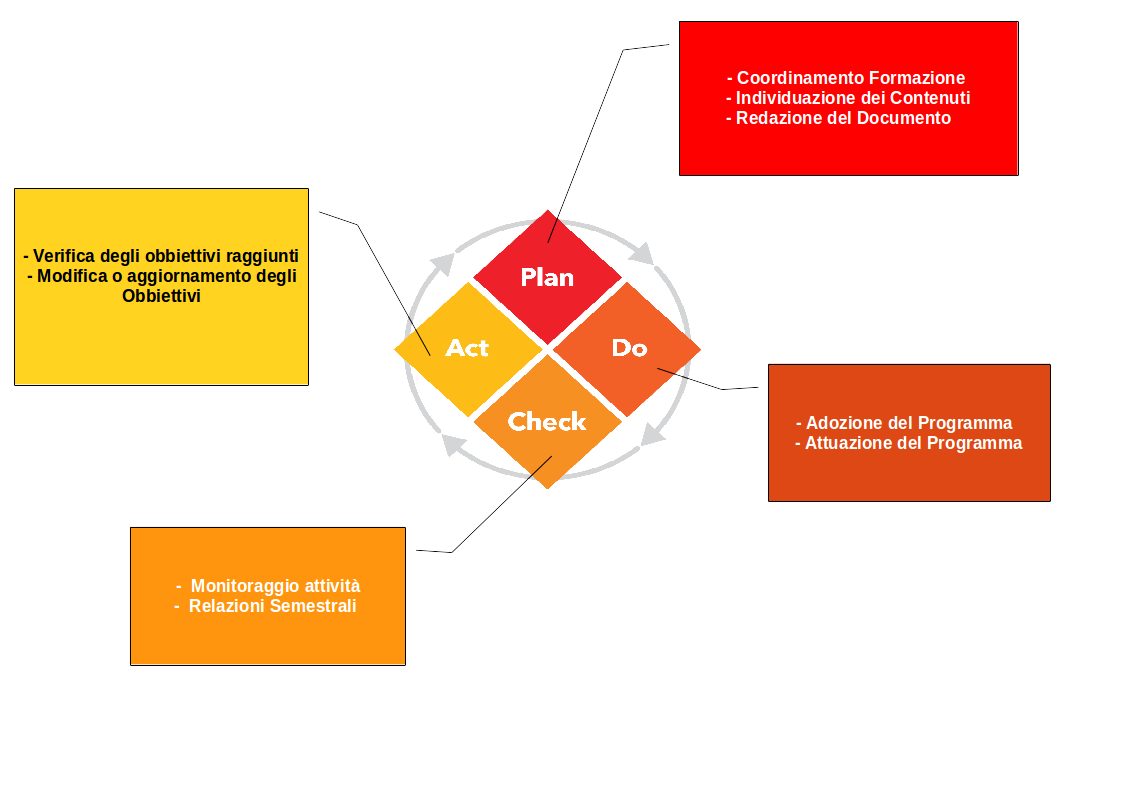
\includegraphics[scale=0.5]{./capitoli/capitolo1/img/demming}
\caption{ciclo di Deming ARPAV}
\end{figure}

La modalità della fase di \textit{Attuazione del programma triennale} sono delegate alle strutture indicate dal Programma. Non è compito della Direzione definire i processi di attuazione dei programmi, ma ad ogni struttura è data libera scelta su come organizzare i propri processi di sviluppo. \\

\subsection{Metodologie di Supporto ai Processi}


L'attitudine a svolgere progetti su piani pluriennali non mi ha reso semplice comprendere la tipologia di processo attuato all'interno della sede dello \textit{stage}. Durante la mia partecipazione come stagista, ho capito che vengono sistematicamente svolte attività di \textit{Analisi dei Requisiti}, \textit{Progettazione}, \textit{Test e Rilascio} e \textit{Manutenzione}. 
\begin{figure}[htbp]

	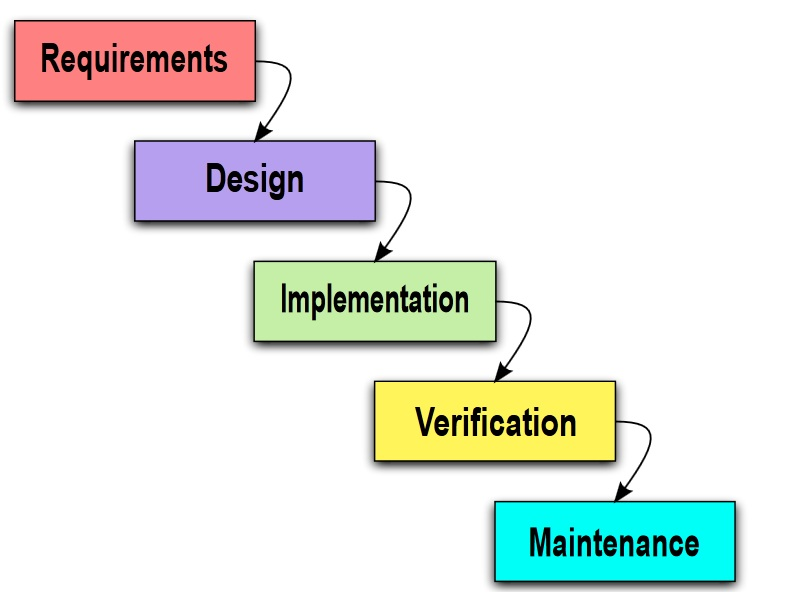
\includegraphics[scale=0.3]{./capitoli/capitolo1/img/cascata}
	\caption{ciclo di vita a cascata}

\end{figure}

Lavorare a progetti che prevedono una durata di sviluppo su base annuale, richiedono una ottima identificazione dei problemi, progettazione di partenza. L'utilizzo di documentazione risulta essenziale, poiché è probabile che subentrino nuove persone all'interno del progetto.
Ne ho dedotto dunque che il ciclo di vita assunto dal dipartimento di informatica è un modello a cascata.


\subsection{Strumenti di Supporto ai Processi}

\subsubsection{Gestione Documenti}
La documentazione riguardante l'analisi dei requisiti viene raccolta all'interno dei server dedicati tramite il \textit{network} da loro gestito. Per altri documenti vengono molto utilizzati servizi come \textit{Google Drive}. 
 


\subsubsection{Ticketing}

Durante la mia presenza in sede ho potuto notare come gli strumenti di \textit{ticketing} fossero utilizzati in parte. Nonostante fossero presenti erano comunque necessarie riunioni per conoscere la situazione interna dei progetti.
\subsubsection{Gestione Calendario}

Per la gestione delle attività di gruppo, come riunioni ufficiali per il resoconto delle attività o la risoluzione di conflitti interni, viene utilizzato lo strumento \textit{Google Calendar}.




\section{Relazioni Esterne}


Essendo un'agenzia regionale finalizzata al monitoraggio e alla tutela dell'ambiente, ARPAV non ha un vero e proprio \textit{target} di clientela. \\
A seconda del ruolo che l'agenzia ricopre in un progetto (\textit{patner} o \textit{leader}) può collaborare con altre agenzie o aziende per fornire prodotti o migliorare infrastrutture. Altrimenti, attraverso i suoi servizi, può interfacciarsi con le singole imprese, industrie e  privati cittadini. 

\subsection{Orientamento all'Innovazione}
Gli obiettivi di ARPAV sono:
\begin{itemize}
	
\item    \textbf{la protezione}, attraverso i controlli ambientali che tutelano la salute della popolazione e la sicurezza del territorio;
\item \textbf{la prevenzione}, attraverso la ricerca, la formazione, l'informazione e l'educazione ambientale.
\end{itemize} 

L'innovazione nelle tecnologie, nei servizi e nelle infrastrutture portano ad un continuo raggiungimento dei due obiettivi preposti. ARPAV non ha come fine un guadagno, ma è un'agenzia regionale che è stata istituita per migliorare la qualità dell'ambiente che ci circonda e quindi la vita. Tramite processi di innovazione l'agenzia sarà in grado di: 
\begin{itemize}
	\item ridurre i costi dei propri servizi;
	\item diminuire i danni ambientali presenti;
	\item monitorare il territorio per la prevenzione dei rischi;
	\item fornire una rapida ed efficace risposta in caso di necessità.
	
\end{itemize}

